\section*{Appendix C: Supplemental Figures}

\renewcommand{\thefigure}{C\arabic{figure}}
\renewcommand{\theequation}{C\arabic{equation}}
\renewcommand{\thetable}{C\arabic{table}}
\setcounter{equation}{0}
\setcounter{figure}{0}
\setcounter{table}{0}


\begin{figure}[ht!]
\centering
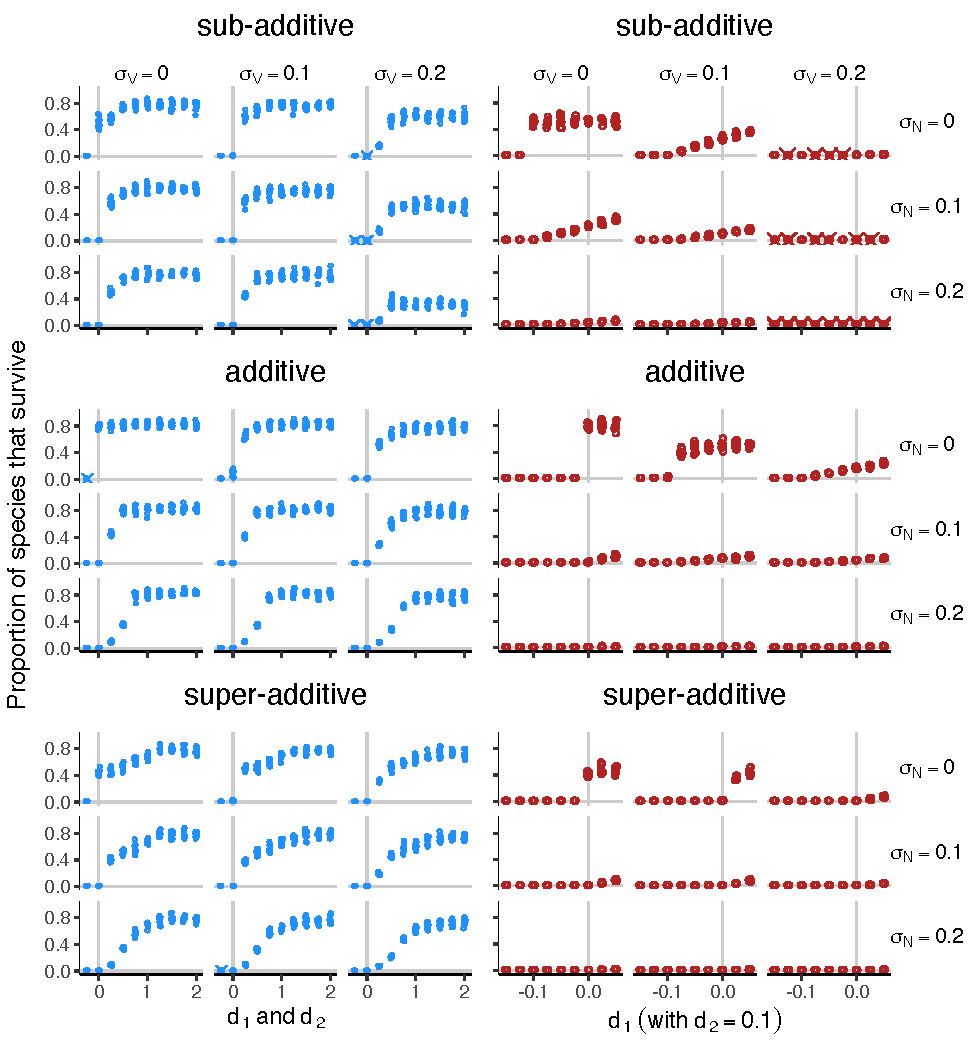
\includegraphics[width=0.9\textwidth]{S3-stoch_coexist.pdf}
\caption{Proportion of species that survived in simulations of 100-species, 2-trait
    communities with
    (A) varying $d_1$ and $d_2$ or 
    (B) varying just $d_1$ with $d_2$ fixed at 0.1.
    Standard deviations are for stochasticity in
    population dynamics ($\sigma_N$) and
    trait evolution ($\sigma_V$).
    Shown for sub-additive ($\eta < 0$), additive ($\eta = 0$), and 
    super-additive ($\eta > 0$) tradeoffs.
    Additive genetic variance ($\sigma_i^2$) was fixed at 0.05 for 
    these simulations.}
\label{fig:stoch-coexist-nspp}
\end{figure}



\begin{figure}[ht!]
\centering
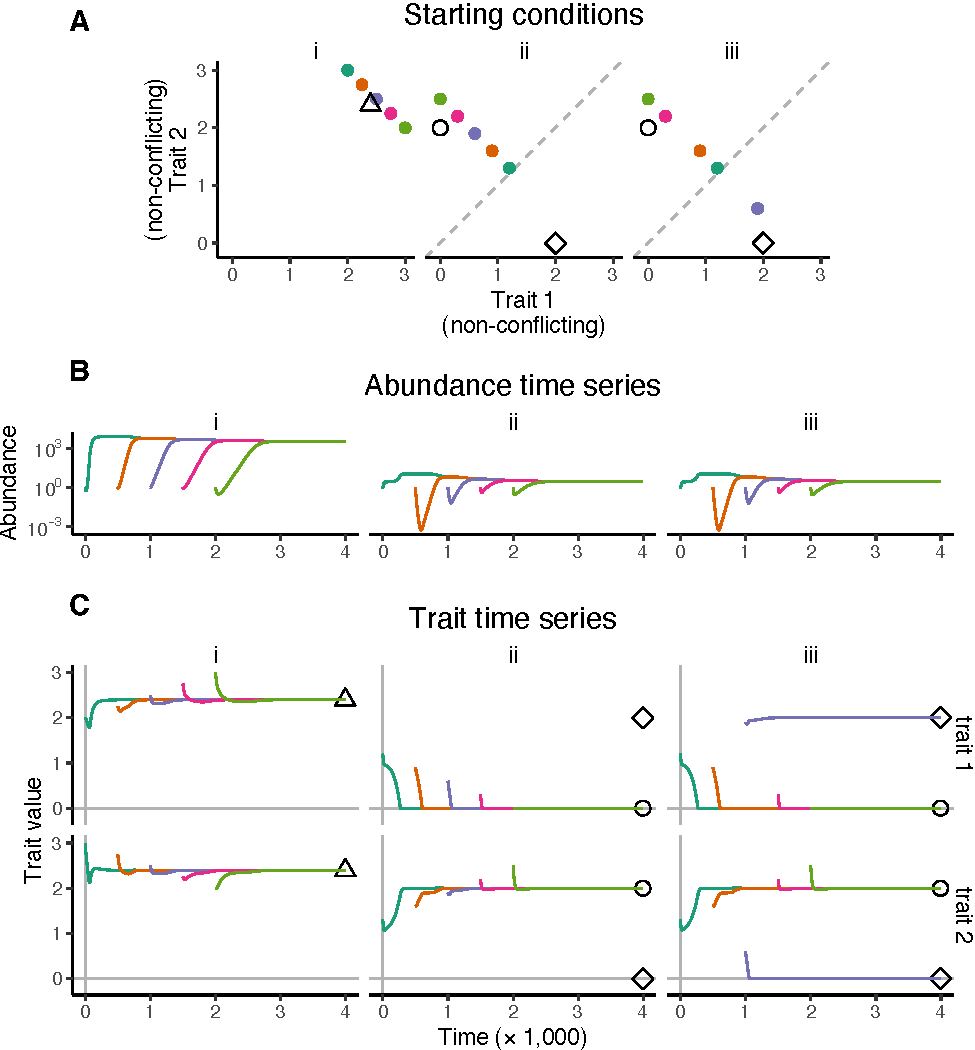
\includegraphics[width=0.7\textwidth]{S1-cond_coexist_non-conflicting.pdf}
\caption{Coexistence for 2-trait, 5-species communities when
    both traits have non-conflicting evolution.
    Panels show, for each of five situations,
    (A) starting conditions and trajectories for each species in trait space, 
    (B) abundances through time, and 
    (C) trait values through time.
    Situation i has sub-additive tradeoffs, situations ii and iv have 
    super-additive, and iii and v have additive.
    (A) Dashed arcs show the location of neutrally stable rings
    when tradeoffs are additive, and 
    the dotted lines separate the basins of attraction for the two possible
    trait states when tradeoffs are super-additive.
    (A,C) Shapes of hollow points indicate the equilibrium trait state.
    (C) For situations iii and v, line width is proportional to the 
    distance from the neutrally stable ring.}
\label{fig:cond-coexist-non-conflicting}
\end{figure}


\begin{figure}[ht!]
\centering
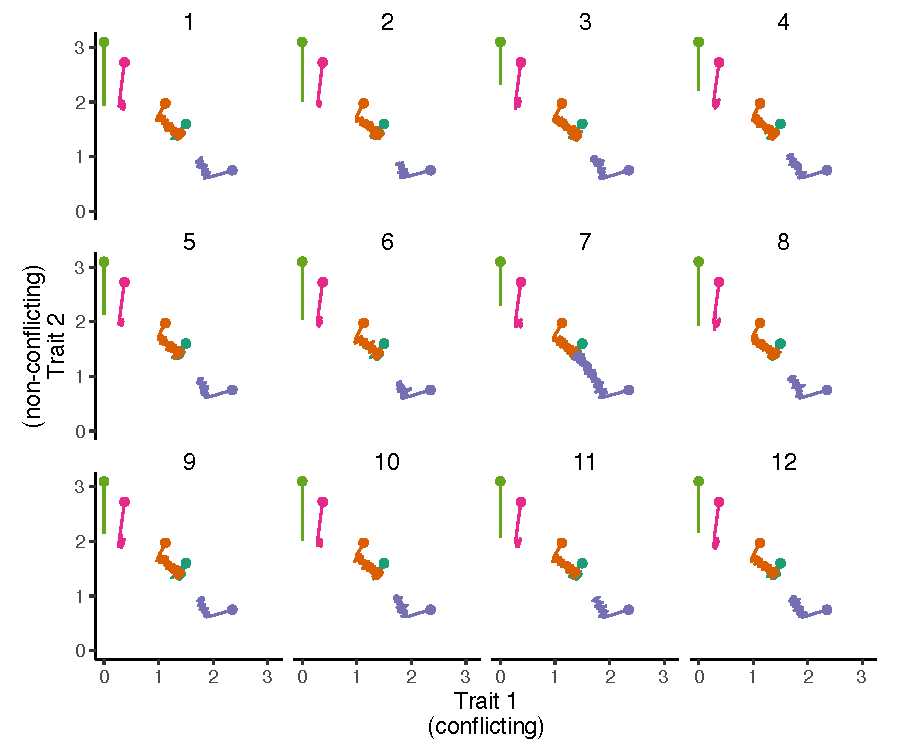
\includegraphics{S2-cc_sigmaV_sit_v.pdf}
\caption{Genotype trajectories through trait space for 12 repetitions under 
scenario v (see main text), with trait stochasticity ($\sigma_V = 0.1$).
Points indicate starting locations, and color indicates species.}
\label{fig:cond-coexist-Vstoch-sit-v}
\end{figure}



\begin{figure}[ht!]
\centering
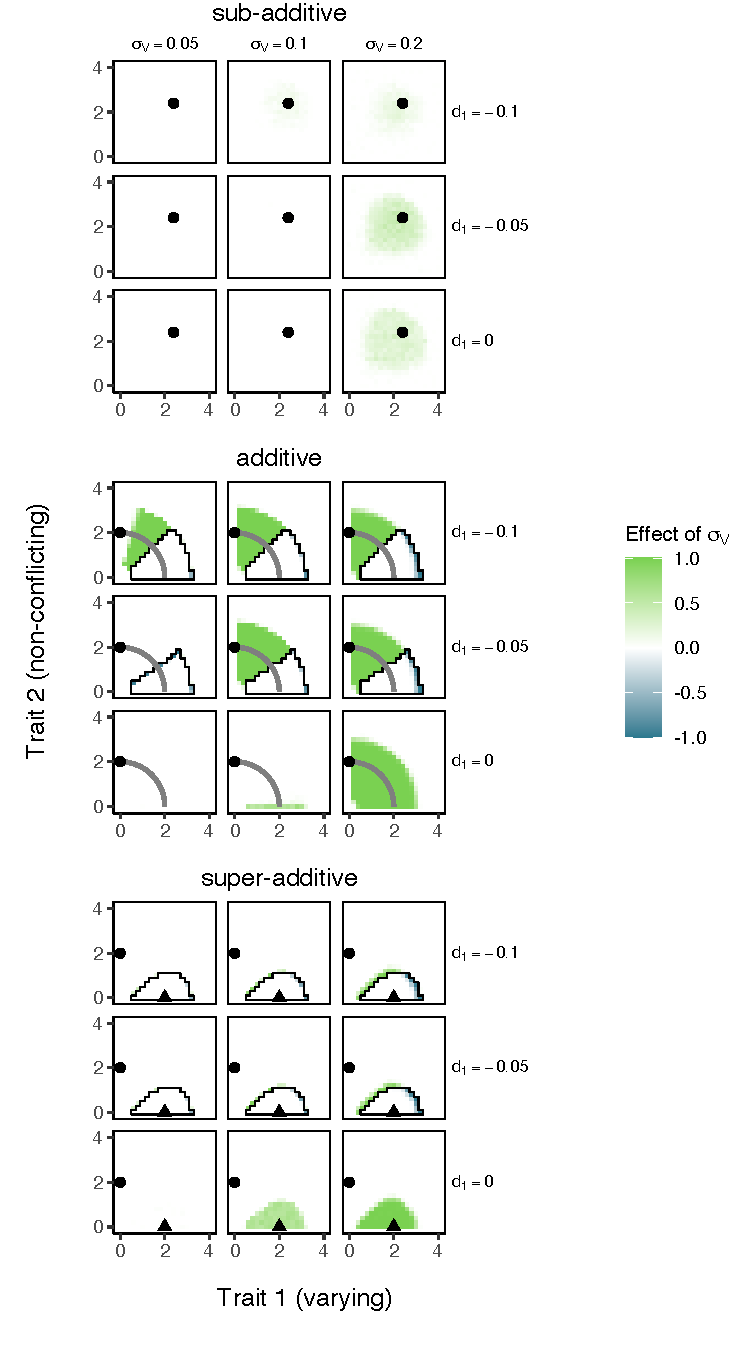
\includegraphics[width=0.5\textwidth]{S4-inv_sims_hm_replace.pdf}
\caption{Effect of stochasticity on replacement of resident species by invader
    based on the invader's starting trait values (x and y axes),
    magnitude of stochasticity (sub-panel columns), and 
    value of $d_1$ (sub-panel rows).
    Shown for sub-additive, additive, and super-additive tradeoffs.}
\label{fig:inv-sims-heatmap-replace}
\end{figure}

\begin{figure}[ht!]
\centering
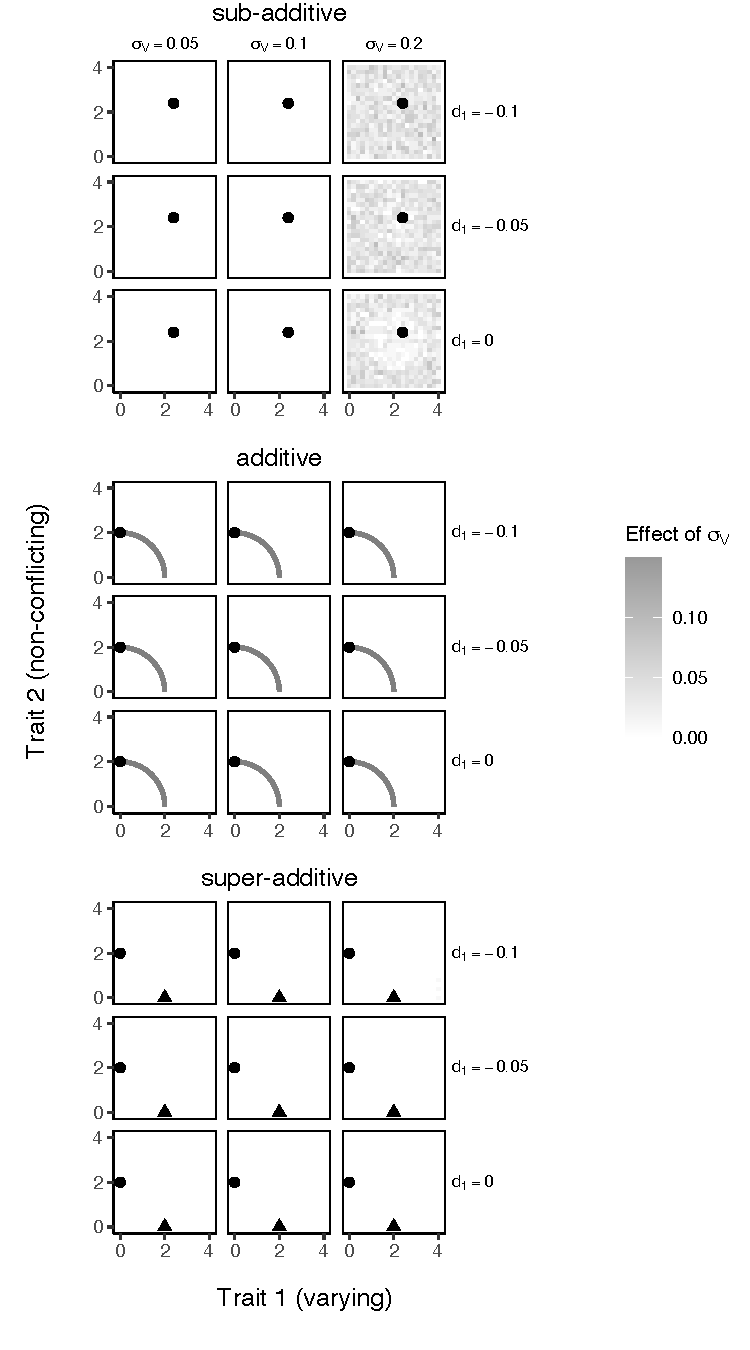
\includegraphics[width=0.5\textwidth]{S5-inv_sims_hm_extinct.pdf}
\caption{Effect of stochasticity on extinction of both resident and invader
    species based on the invader's starting trait values (x and y axes),
    magnitude of stochasticity (sub-panel columns), and 
    value of $d_1$ (sub-panel rows).
    Shown for sub-additive, additive, and super-additive tradeoffs.}
\label{fig:inv-sims-heatmap-extinct}
\end{figure}

